\chapter{Classification networks}
\label{chapt:cnets}
In order to better understand the detection networks, we will shortly describe their predecessors, classification networks. Classification network is a convolutional neural network (CNN) \cite[ch.~9]{bib:dlbook} which given an image, returns a confidence score of correspondence to each of the classes. 
In \cref{chapt:models} we will see that the classification models are used as a backbone for the detectors.

\subsection*{AlexNet (2012)}
A significant breakthrough in use of CNNs happened in 2012, when the \textit{AlexNet} \cite{bib:alexnet} won the \textit{ImageNet} image recognition challenge\footnote{\url{http://www.image-net.org/challenges/LSVRC/}} with deep CNN against traditional computer vision and machine learning approaches. AlexNet has a simple architecture with five convolutional layers and two fully connected layers followed by a softmax layer. It created a foundation on which today's state-of-the-art models are build.

\subsection*{VGG (2014)}
\label{sec:VGG}
The network architecture, mostly known as VGG, comes from the \textit{Very Deep Convolutional Networks for Large-Scale Image Recognition} paper \cite{bib:vgg} by \textit{Visual Geometry Group}\footnote{\url{http://www.robots.ox.ac.uk/~vgg/}} and it pushed the concept of AlexNet even further and proved the feasibility of deeper network with small convolutions. Each of the VGG's convolutional filters use 3 by 3 kernel and the depth of the filters increases throught the network. After the convolutions, three fully connected layers and softmax are applied. The exact architecture is described in \cref{tab:vgg_arch}. VGG network is considered a general architecture for a classifier network. 

\begin{table}[]
    \label{tab:vgg_arch}
    \centering
    \rotatebox{90}{
        \vggArch
    }
    \caption{Architecture of VGG network, version D. Taken from \cite[table 1]{bib:vgg}}
\end{table}
    
\subsection*{Inception v1 (2014)}
\label{sec:inception}
Also called GoogLeNet
mention v2,3,4

\subsection*{ResNet (2015)}
\label{sec:resnet}

All ResNet \cite{bib:resnet} architectures (ResNet-10, ResNet-18, 34, 50...) use the same architecture (left chart), which is build from a few input layers, four sets of building blocks and output layers. Each of four blocks can be composed of multiple residual building blocks. There are two types of building blocks, larger block with three convolutional layers called "bottleneck", or smaller "basic" block with two convolutional layers.  see \cref{fig:resnet_arch}

\begin{figure}
    \label{fig:resnet_arch}
    \resnetArch
    \caption{Architecture of ResNet network.
    Note that the give number of convolutional filters in building blocks depends on which block do they belong to. For more detailed specification see Table 1 in  \cite{bib:resnet}.}
\end{figure}

\subsection*{NasNet (2017)}
\label{sec:nasnet}

\begin{figure}
    \label{fig:cnncomp}
    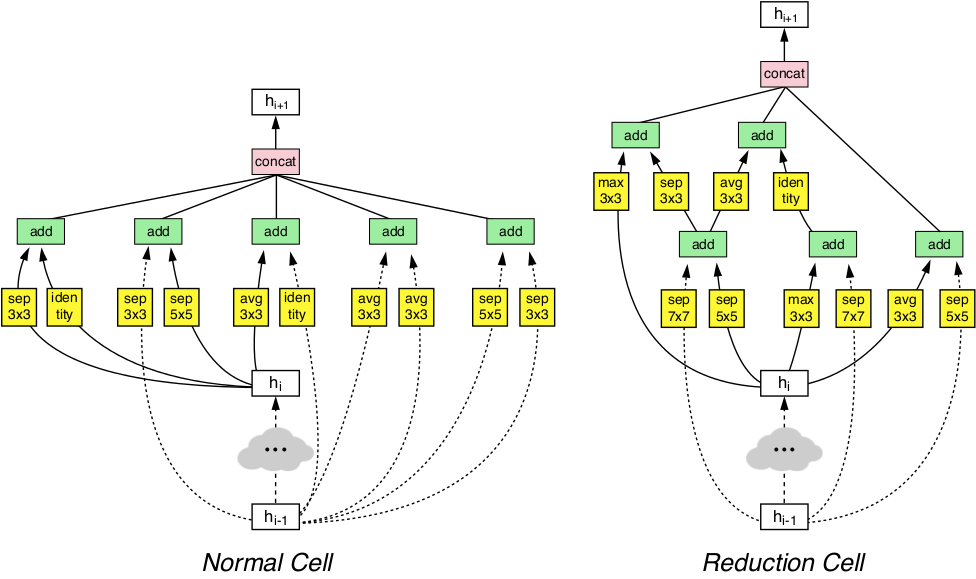
\includegraphics[width=\textwidth]{img/nasnet}
    \caption{Accuracy versus computational demand across top performing published CNN architectures on ImageNet 2012 ILSVRC challenge prediction task. Computational demand is measured in the number of floating-point multiply-add operations to process a single image. Taken from \cite{bib:nasnet}.}
\end{figure}





